\begin{figure}[!htbp]
\caption{Representative Ideal Points and District Ideology (Three Groups)}
\begin{centering}
%\centering
%\fbox{
  \begin{tabular}{@{}cc@{}}
	 & \\  	
	\small (A) Marginal Effect of Percent Same-Party&	
  	\small (B) Marginal Effect of Same-Party Ideology\\
    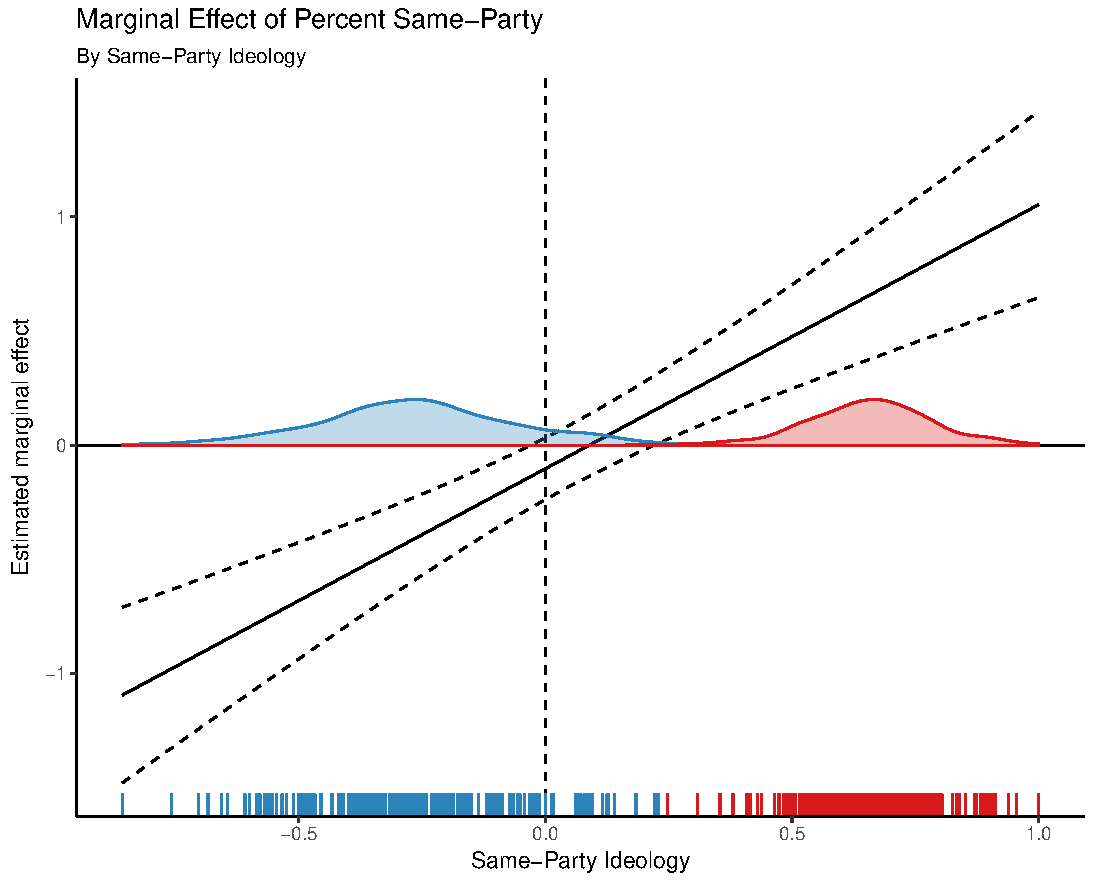
\includegraphics[width=.45\textwidth]{/Users/dsimp/GitHub/Clinton(2006)Rep/drafts/marginals/meb-1.pdf} &
    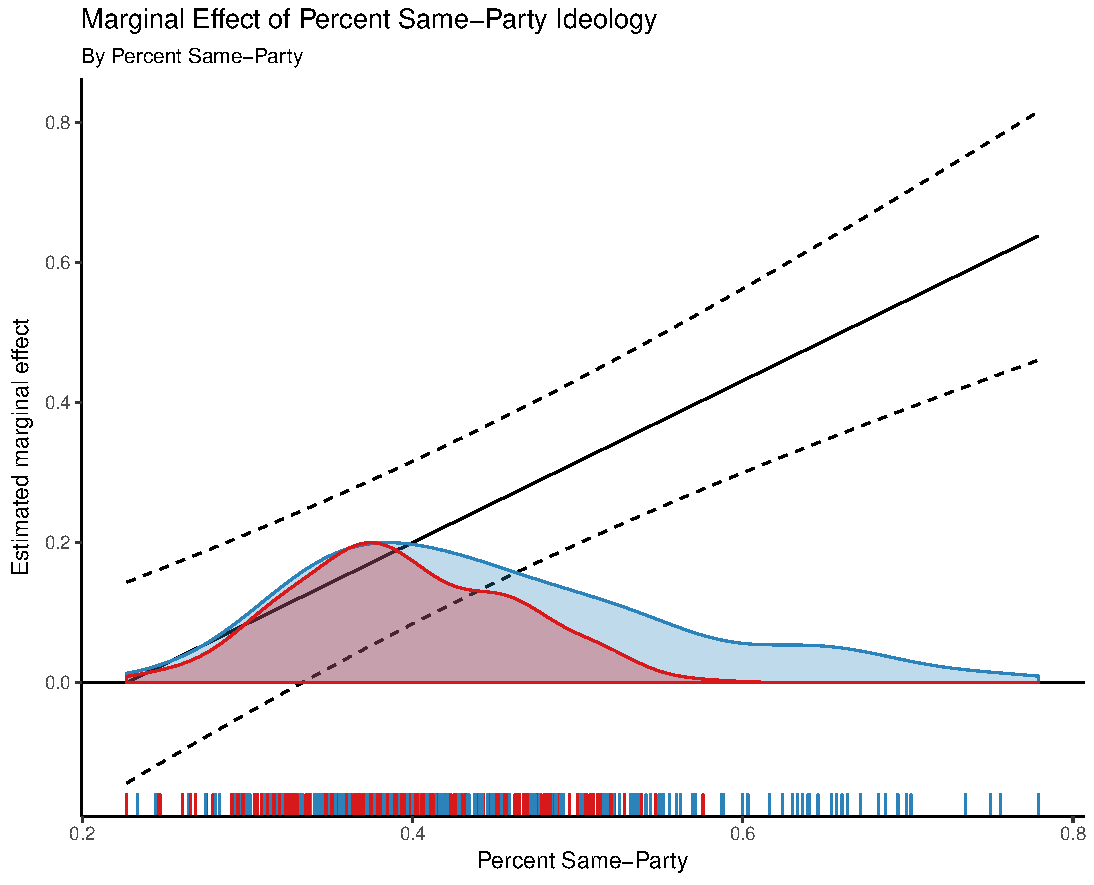
\includegraphics[width=.45\textwidth]{/Users/dsimp/GitHub/Clinton(2006)Rep/drafts/marginals/meb-2.pdf} \\
     & \\
	\small (C) Marginal Effect of Percent Independent& 
    \small (D) Marginal Effect of Independent Ideology\\
    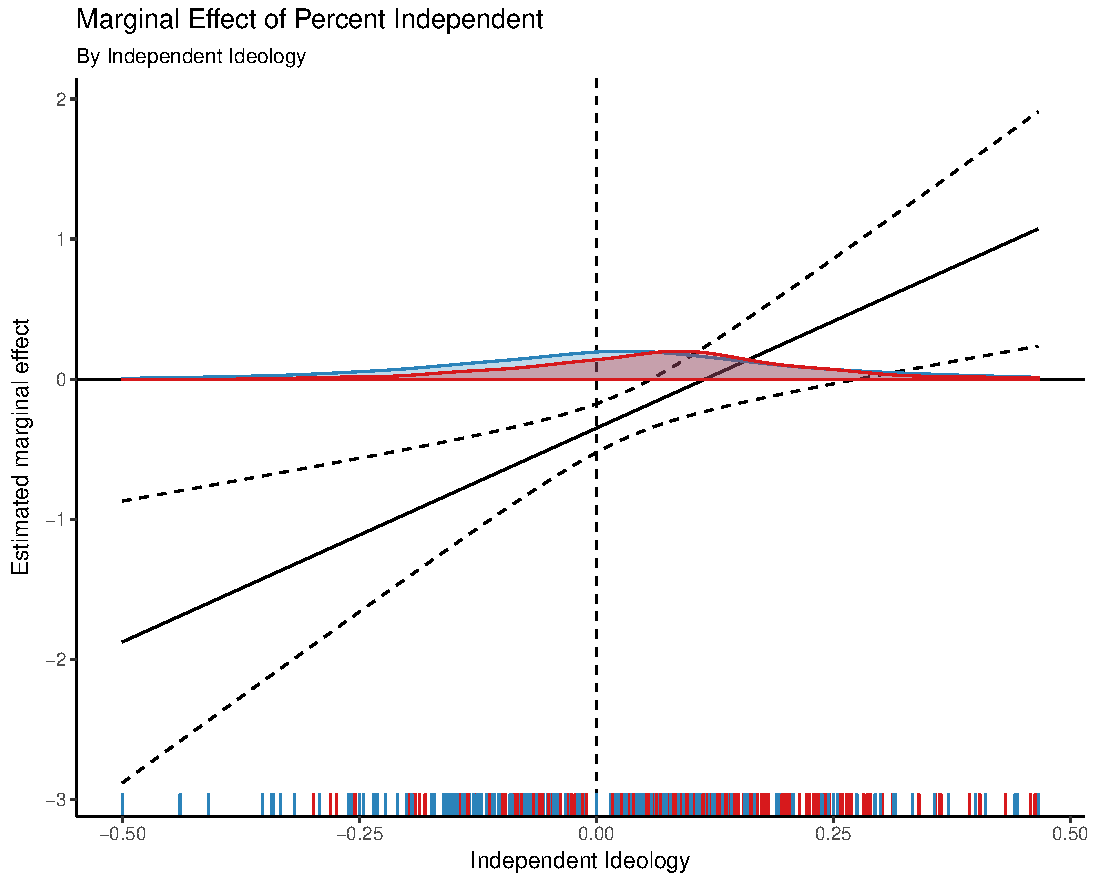
\includegraphics[width=.45\textwidth]{/Users/dsimp/GitHub/Clinton(2006)Rep/drafts/marginals/meb-3.pdf} &
    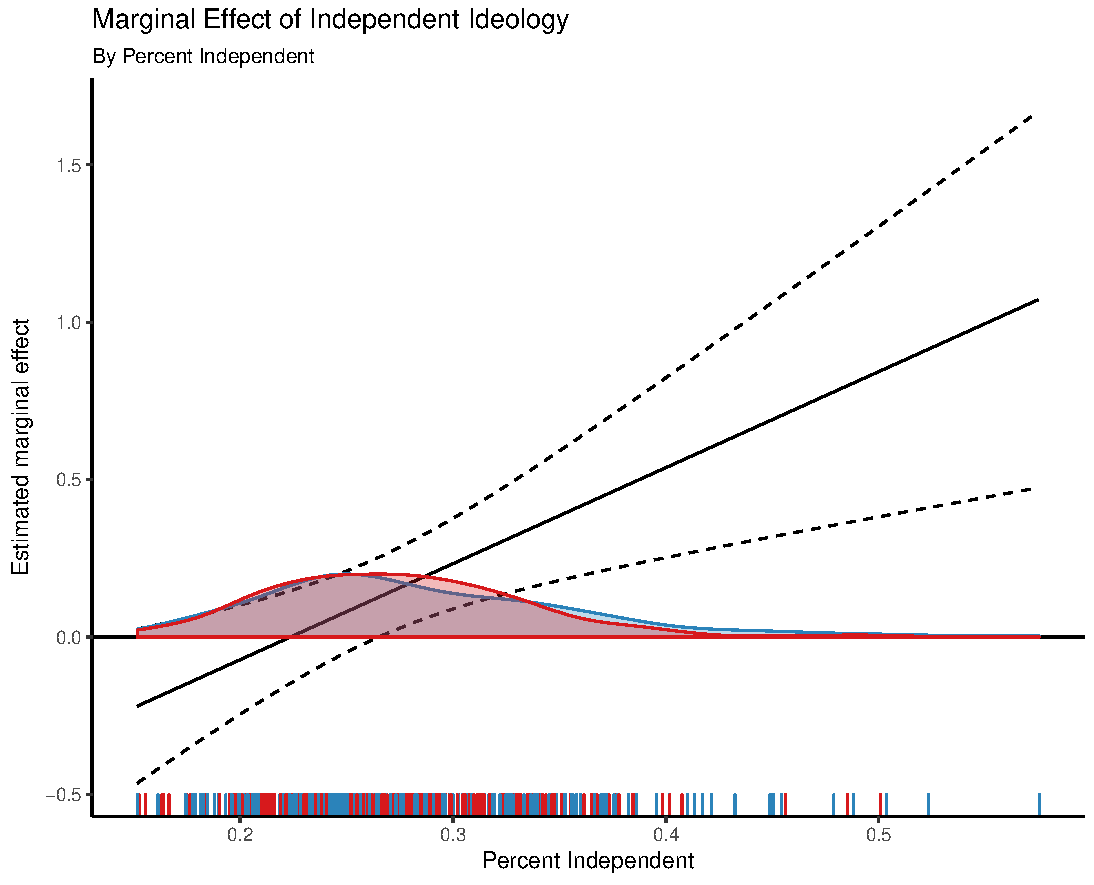
\includegraphics[width=.45\textwidth]{/Users/dsimp/GitHub/Clinton(2006)Rep/drafts/marginals/meb-4.pdf} \\
     &  \\
    \small (E) Marginal Effect of Percent Opposite-Party&  
    \small (F) Marginal Effect of Opposite-Party Ideology\\
    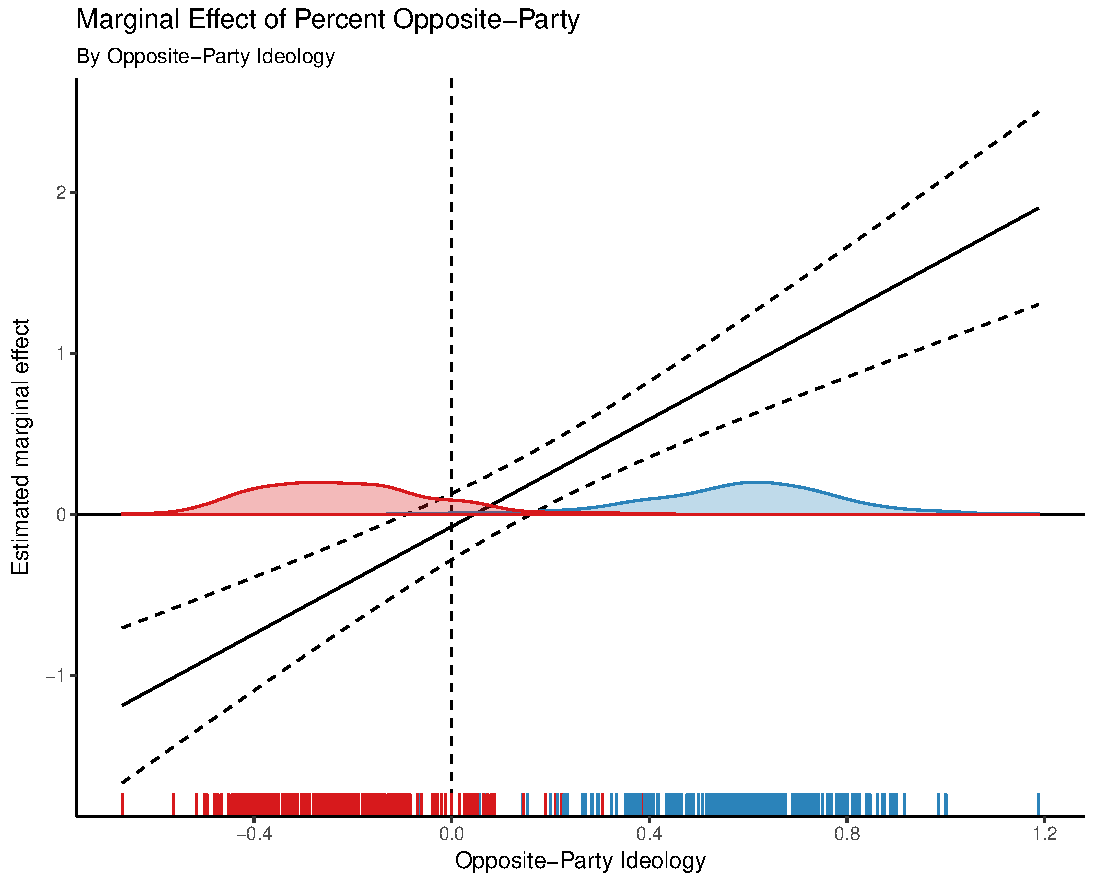
\includegraphics[width=.45\textwidth]{/Users/dsimp/GitHub/Clinton(2006)Rep/drafts/marginals/meb-5.pdf} &
    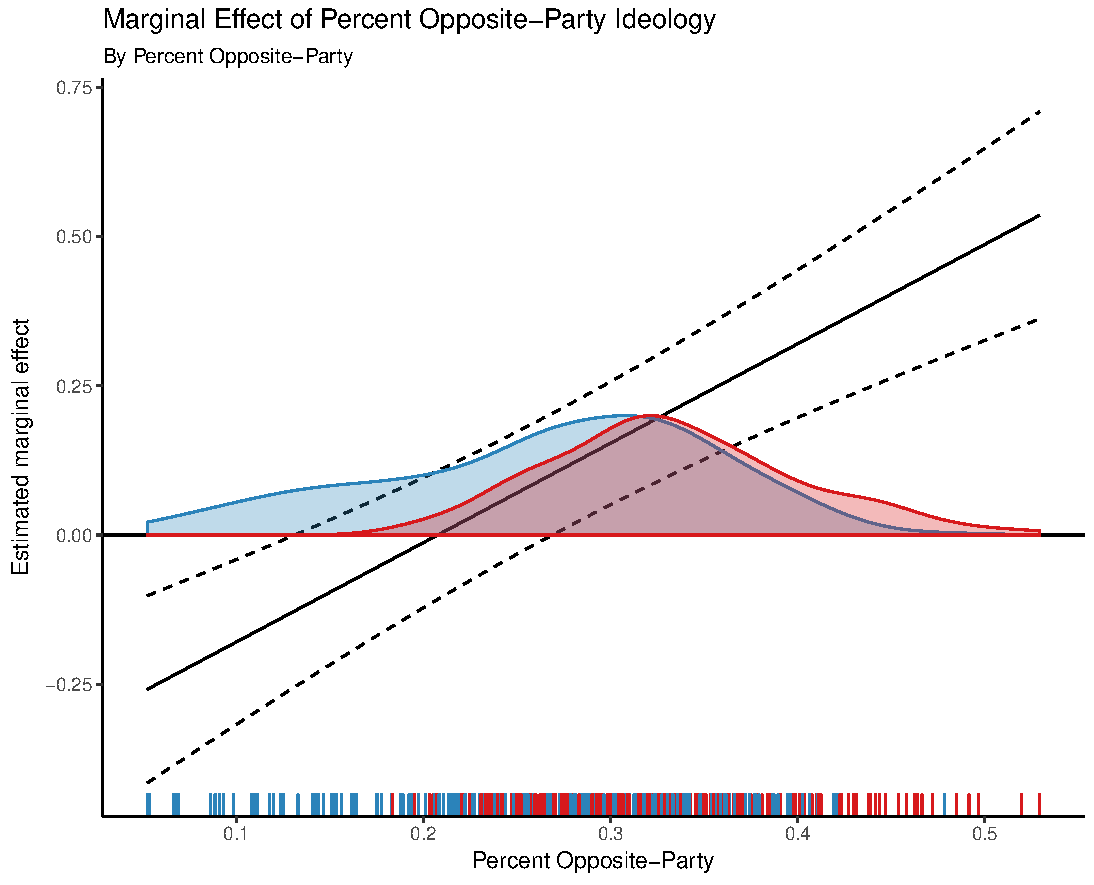
\includegraphics[width=.45\textwidth]{/Users/dsimp/GitHub/Clinton(2006)Rep/drafts/marginals/meb-6.pdf} \\
     &  \\
  \end{tabular}
    %}   
 \end{centering}
  \textbf{Note:} Each panel plots the respective marginal effect of the constitutive terms of the interaction variables in Table 2 Model 5.
\end{figure}
